\section{HOHS Data Characteristics and Problem Formulation}\label{sec:problem formulation}

This section characterizes the HOHS datasets and formulates the data-reduction problem considered in this work.

\subsection{Characterizing HOHS Simulation Datasets}\label{sec:problem formulation:data characteristics}

In general, HOHS datasets can have different formats depending on the simulation framework. For example, NekRS~\cite{fischer2022nekrs} stores multiple physical fields in a single binary file, while MFEM~\cite{kolev2010modular} represents mesh information and field data in separate plain-text files. Nektar++~\cite{moxey2020nektar++} stores simulation outputs in a native binary format that is not directly readable and requires conversion to VTU using its accompanying conversion tool before visualization and analysis. Despite these differences in storage formats, such datasets share common characteristics intrinsic to spectral element methods.

From a global perspective, data points are organized as a collection of geometrically deformed hexahedral elements connected through shared faces in an unstructured manner. In cases where the simulation is defined on a surface, the elements are deformed quadrilateral and connected through shared edges. Figure~\ref{fig:characterizing-hohs}(a) illustrates a simple example in which three hexahedral elements are connected pairwise, forming a mesh that does not follow a regular tiling pattern. Such irregular adjacencies are common in HOHS datasets.

\begin{figure}[htb]
    \centering
    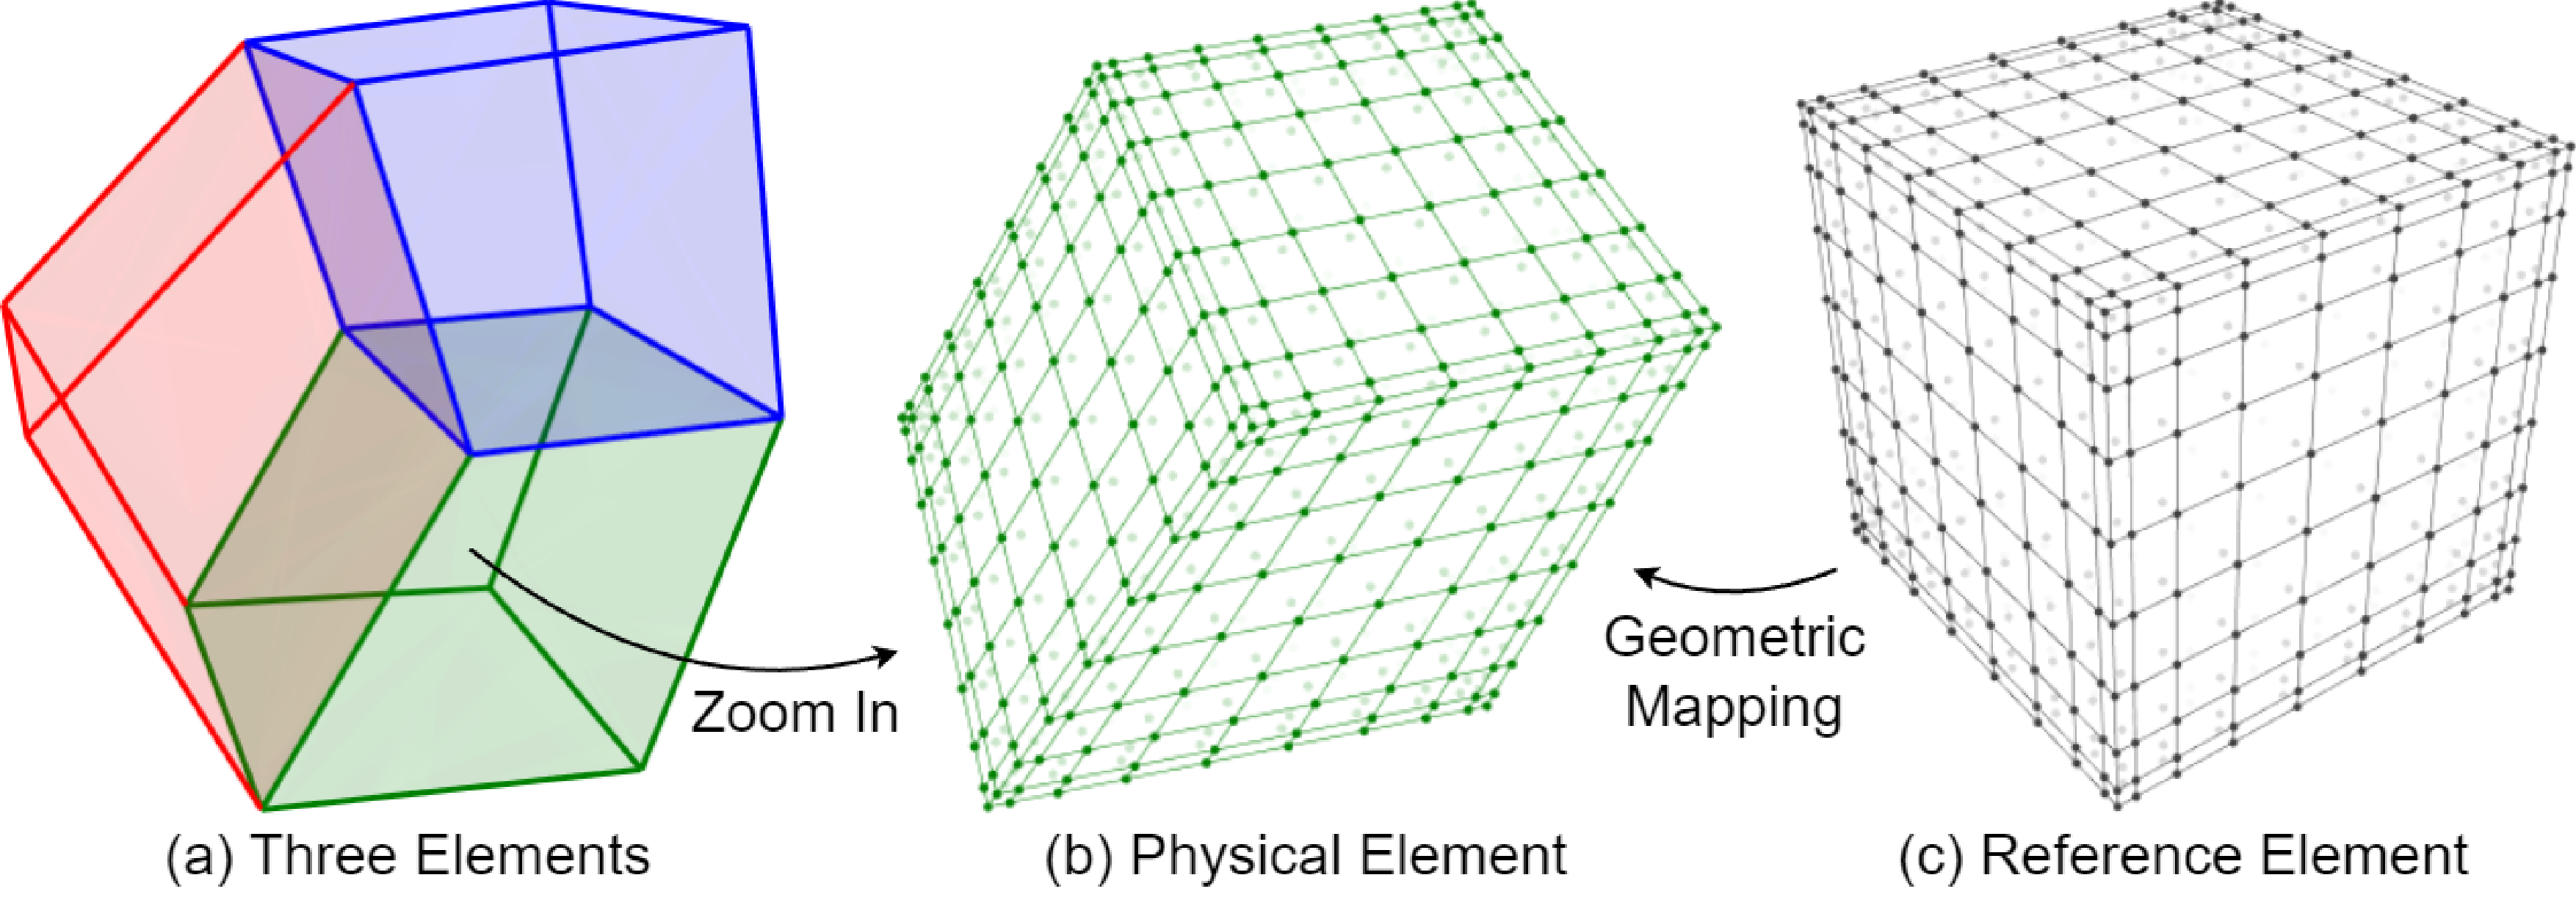
\includegraphics[width=\linewidth]{figs/3/three_elements.pdf}
    \caption{Hybrid organization of HOHS datasets. (a) Globally, physical elements exhibit irregular inter-element connectivity. (b) Locally, each physical element contains a deformed tensor-product grid of data points. (c) These physical elements are obtained by geometrically mapping a common fixed reference element.}
    \label{fig:characterizing-hohs}
\end{figure}

At a local scale, the HOHS data exhibit a markedly different structure. Within each element, the number of data points is fixed and identical for all elements. These points are arranged in a deformed tensor-product layout, typically forming an $n \times n \times n$ grid. Figure~\ref{fig:characterizing-hohs}(b) illustrates this structure using the green element in Figure~\ref{fig:characterizing-hohs}(a) as an example, which contains $10 \times 10 \times 10$ data points. For visual clarity, the figure highlights the data points close to the three visible faces of the element.

For a given element shape, all elements are derived from a common reference element with a canonical shape. Inside the reference element, the coordinates of data points in each dimension take values from a fixed set. In practice, most solvers adopt sets associated with specific high-order polynomial bases due to considerations such as numerical stability, accuracy, and quadrature compatibility. Among these, Gauss-Lobatto-Legendre (GLL) points are particularly common because they enable accurate numerical quadrature for high-order polynomial integrands while including the element boundaries. Figure~\ref{fig:characterizing-hohs}(c) illustrates the GLL node distribution in the reference element. The data points shown in Figure~\ref{fig:characterizing-hohs}(b) can be viewed as a physical-space mapping of this reference element. Although alternative sets may be supported, our examination of several representative frameworks shows that GLL points are consistently used under default settings.

During simulation, data values are first computed in the reference element and subsequently mapped to their corresponding locations in physical spaces. 
The deterministic element-local point distributions and data generation process are key to the compression design proposed in this work.

\subsection{Problem Formulation}

\begin{figure}[htb]
    \centering
    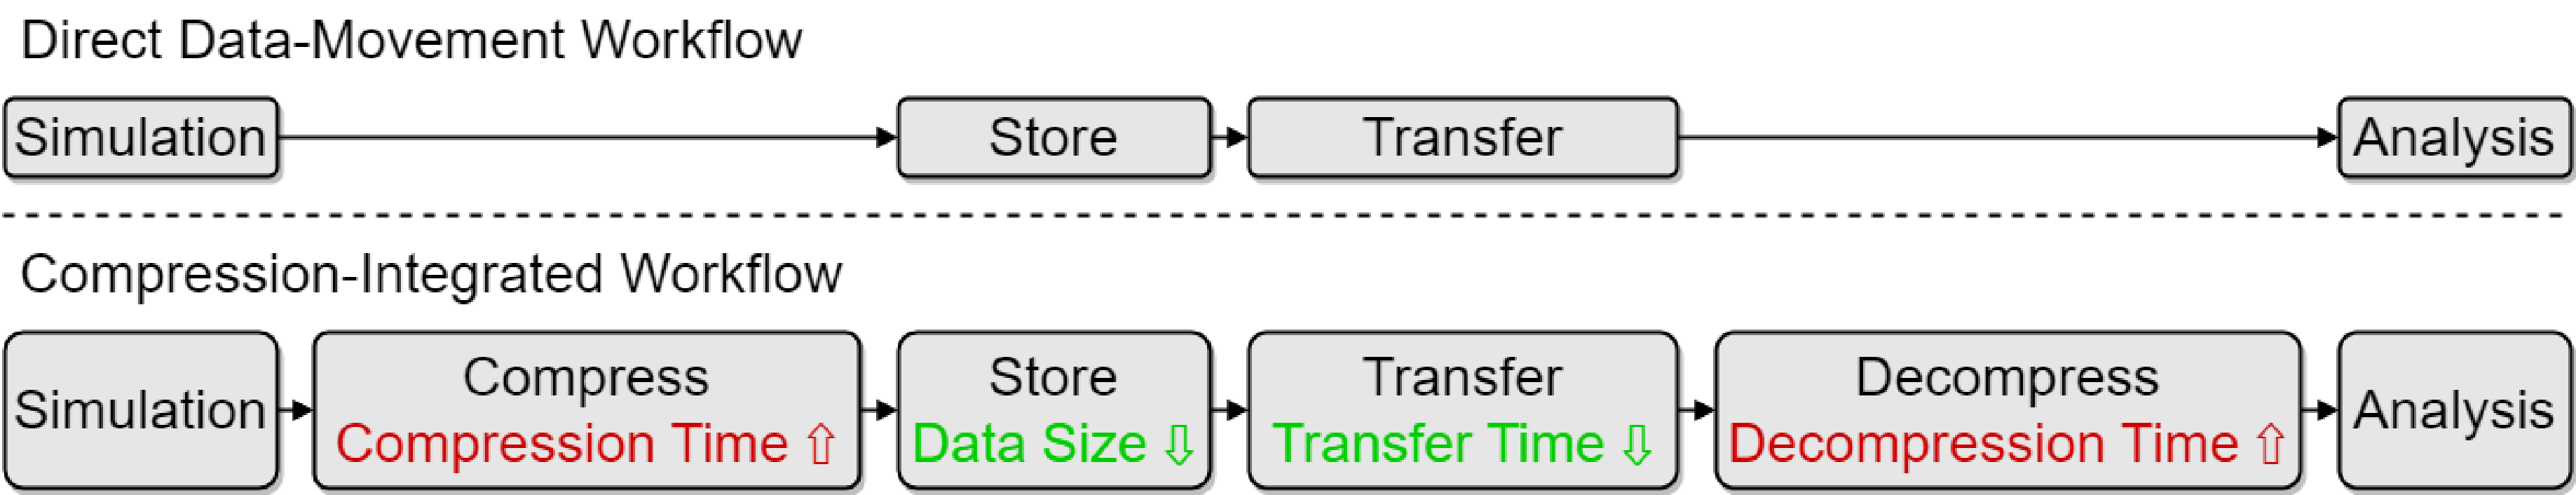
\includegraphics[width=1\linewidth]{figs/3/End to End.pdf}
    \caption{Compression-Integrated Data-Management Workflow}
    \label{fig:end-to-end}
\end{figure}

In this work, we use compressors to improve HOHS data management, but their effectiveness is non-trivial and must be evaluated from multiple perspectives. As illustrated in Figure~\ref{fig:end-to-end}, compression often reduces storage footprint and transfer volume, but it also introduces compression and decompression overhead. Ideally, a data-reduction method would provide a high compression ratio with negligible computational overhead, thereby reducing end-to-end data-movement time. In practice, however, higher compression ratios often require more sophisticated algorithms and longer computation time.

In this paper, we evaluate HOHS data reduction along two primary dimensions: the storage footprint of the reduced data under comparable data quality, and the overall end-to-end time required for compression, data movement, and decompression. These dimensions are assessed through three evaluation metrics.
\begin{itemize}
    \item \textbf{\textit{Data Quality}} characterizes the fidelity of reconstructed simulation data. It can be quantified using numerical metrics such as the prescribed upper error bound and peak signal-to-noise ratio (\textit{PSNR}). While these metrics provide convenient numerical measures, domain scientists often place greater emphasis on the \textit{visual fidelity} of simulation results. Accordingly, we also assess reconstruction quality through visualization-based evaluations, which are presented in Section~\ref{sec:performance evaluation:visualization}.
    \item \textbf{\textit{Storage Reduction}} measures the reduced storage footprint achieved under a given data-quality constraint. We report this using either the \textit{compression ratio} or the \textit{bit rate}. The compression ratio is defined as the size of the original data divided by the size of the compressed representation, whereas the bit rate denotes the average number of bits required per data value after reduction. These two metrics provide equivalent views of storage efficiency.
    \item \textbf{\textit{End-to-End Runtime}} measures the net practical cost of using data reduction in realistic data-movement workflows. We evaluate the total time required for compression, network transmission of the reduced data via Globus, and decompression.
\end{itemize}

To make such compression-based data reduction suitable for HOHS data management, the method should satisfy two key requirements.
\begin{itemize}
    \item \textbf{\textit{Field Independence}}: Different physical fields may have different accuracy requirements and downstream analysis semantics. The method should therefore support independent reduction of each field, allowing users to specify field-level quality constraints while avoiding unnecessary coupling across heterogeneous variables.
    \item \textbf{\textit{Error-bound Guarantee}}: The reduction process must satisfy a pointwise error-bound guarantee. Specifically, given a user-specified error bound $\varepsilon$, each reconstructed value must differ from its corresponding original value by no more than $\varepsilon$, under either an absolute or relative error criterion. This guarantee is essential for maintaining the fidelity of downstream scientific analysis.
\end{itemize}